% Kommentare für den Editor (TexWorks/TexMakerX)
% !TeX encoding   = utf8
% !TeX spellcheck = de-DE

% --- LaTeX Vorlage ------------------------------------------------------
% Vorlage für Praktikumsprotokolle in den Modulen Verteilte Systeme, Betriebssysteme
%
% Autor: Aljoscha Pörtner (aljoscha.poertner@fh-bielefeld.de
% ------------------------------------------------------------------------

% Dokumentenklasse (Koma Script) -----------------------------------------
\documentclass[%
   %draft,     % Entwurfsstadium
   final,      % fertiges Dokument
   paper=a4, paper=portrait, pagesize=auto, % Papier Einstellungen
   fontsize=11pt, % Schriftgröße
   ngerman, % Sprache 
 ]{scrartcl} % Classes: scrartcl, scrreprt, scrbook

% ~~~~~~~~~~~~~~~~~~~~~~~~~~~~~~~~~~~~~~~~~~~~~~~~~~~~~~~~~~~~~~~~~~~~~~~~
% encoding
% ~~~~~~~~~~~~~~~~~~~~~~~~~~~~~~~~~~~~~~~~~~~~~~~~~~~~~~~~~~~~~~~~~~~~~~~~

% Encoding der Dateien (sonst funktionieren Umlaute nicht)
\usepackage[utf8]{inputenc}

% Encoding der Verzeichnisse (für Pfade mit Umlauten und Leerzeichne)
\usepackage[%
   extendedchars, encoding, multidot, space,
   filenameencoding=latin1, % Windows XP, Vista, 7
   % filenameencoding=utf8,   % Linux, OS X
]{grffile}
\usepackage{here}
% ~~~~~~~~~~~~~~~~~~~~~~~~~~~~~~~~~~~~~~~~~~~~~~~~~~~~~~~~~~~~~~~~~~~~~~~~
% Pakete und Stile
% ~~~~~~~~~~~~~~~~~~~~~~~~~~~~~~~~~~~~~~~~~~~~~~~~~~~~~~~~~~~~~~~~~~~~~~~~
% Schriften
% ~~~~~~~~~~~~~~~~~~~~~~~~~~~~~~~~~~~~~~~~~~~~~~~~~~~~~~~~~~~~~~~~~~~~~~~~
% Fonts Fonts Fonts
% ~~~~~~~~~~~~~~~~~~~~~~~~~~~~~~~~~~~~~~~~~~~~~~~~~~~~~~~~~~~~~~~~~~~~~~~~

% immer laden:
\usepackage[T1]{fontenc} % T1 Schrift Encoding
\usepackage{textcomp}	 % Zusätzliche Symbole (Text Companion font extension)

% ~~~~~~~~~~~~~~~~~~~~~~~~~~~~~~~~~~~~~~~~~~~~~~~~~~~~~~~~~~~~~~~~~~~~~~~~
% Symbole
% ~~~~~~~~~~~~~~~~~~~~~~~~~~~~~~~~~~~~~~~~~~~~~~~~~~~~~~~~~~~~~~~~~~~~~~~~

\usepackage{amssymb}
\usepackage{mathcomp}


%% ==== Zusammengesetzte Schriften  (Sans + Serif) =======================

%% - Latin Modern
\usepackage{lmodern}
%% -------------------

%% - Bera Schriften
%\usepackage{bera}
%% -------------------

%% - Times, Helvetica, Courier (Word Standard...)
%\usepackage{mathptmx}
%\usepackage[scaled=.90]{helvet}
%\usepackage{courier}
%% -------------------

%% - Palantino , Helvetica, Courier
%\usepackage{mathpazo}
%\usepackage[scaled=.95]{helvet}
%\usepackage{courier}
%% -------------------

%% - Charter, Bera Sans
%\usepackage{charter}\linespread{1.05}
%\renewcommand{\sfdefault}{fvs}
%\usepackage[charter]{mathdesign}



%%%% =========== Typewriter =============

%\usepackage{courier}                   %% --- Courier
%\renewcommand{\ttdefault}{cmtl}        %% --- CmBright Typewriter Font
%\usepackage[%                          %% --- Luxi Mono (Typewriter)
%   scaled=0.9
%]{luximono}



% Pakete Laden
% ~~~~~~~~~~~~~~~~~~~~~~~~~~~~~~~~~~~~~~~~~~~~~~~~~~~~~~~~~~~~~~~~~~~~~~~~
% These packages must be loaded before all others
% (primarily because they are required by other packages)
% ~~~~~~~~~~~~~~~~~~~~~~~~~~~~~~~~~~~~~~~~~~~~~~~~~~~~~~~~~~~~~~~~~~~~~~~~
\usepackage{calc}
\usepackage{fixltx2e}	% Fix known LaTeX2e bugs

\usepackage[ngerman]{babel} 			% Sprache
\usepackage[dvipsnames, table]{xcolor} 	% Farben

% ~~~~~~~~~~~~~~~~~~~~~~~~~~~~~~~~~~~~~~~~~~~~~~~~~~~~~~~~~~~~~~~~~~~~~~~~
% Bilder, Gleitumgebungen und Platzierung
% ~~~~~~~~~~~~~~~~~~~~~~~~~~~~~~~~~~~~~~~~~~~~~~~~~~~~~~~~~~~~~~~~~~~~~~~~

\usepackage[]{graphicx}					% Graphiken
\usepackage{epstopdf}		% konvertiert eps in pdf

% provides new floats and enables H float modifier option
\usepackage{float}
% Floats immer erst nach der Referenz setzen
\usepackage{flafter}
% Alel Floats werden vor der nächsten section ausgegeben
\usepackage[section]{placeins} 
%

% ~~~~~~~~~~~~~~~~~~~~~~~~~~~~~~~~~~~~~~~~~~~~~~~~~~~~~~~~~~~~~~~~~~~~~~~~
% Beschriftungen (captions)
% ~~~~~~~~~~~~~~~~~~~~~~~~~~~~~~~~~~~~~~~~~~~~~~~~~~~~~~~~~~~~~~~~~~~~~~~~

\usepackage{caption}
\usepackage{subcaption}

% ~~~~~~~~~~~~~~~~~~~~~~~~~~~~~~~~~~~~~~~~~~~~~~~~~~~~~~~~~~~~~~~~~~~~~~~~
% Math
% ~~~~~~~~~~~~~~~~~~~~~~~~~~~~~~~~~~~~~~~~~~~~~~~~~~~~~~~~~~~~~~~~~~~~~~~~

% Base Math Package
\usepackage[fleqn]{amsmath} 
% Warnt bei Benutzung von Befehlen die mit amsmath inkompatibel sind.
\usepackage[all, error]{onlyamsmath}

% ~~~~~~~~~~~~~~~~~~~~~~~~~~~~~~~~~~~~~~~~~~~~~~~~~~~~~~~~~~~~~~~~~~~~~~~~
% Science
% ~~~~~~~~~~~~~~~~~~~~~~~~~~~~~~~~~~~~~~~~~~~~~~~~~~~~~~~~~~~~~~~~~~~~~~~~

% Einheiten und Zahlenformatierung
\usepackage{siunitx}

% ~~~~~~~~~~~~~~~~~~~~~~~~~~~~~~~~~~~~~~~~~~~~~~~~~~~~~~~~~~~~~~~~~~~~~~~~
% Tables (Tabular)
% ~~~~~~~~~~~~~~~~~~~~~~~~~~~~~~~~~~~~~~~~~~~~~~~~~~~~~~~~~~~~~~~~~~~~~~~~

\usepackage{booktabs}
\usepackage{ltxtable} % Longtable + tabularx

% ~~~~~~~~~~~~~~~~~~~~~~~~~~~~~~~~~~~~~~~~~~~~~~~~~~~~~~~~~~~~~~~~~~~~~~~~
% text related packages
% ~~~~~~~~~~~~~~~~~~~~~~~~~~~~~~~~~~~~~~~~~~~~~~~~~~~~~~~~~~~~~~~~~~~~~~~~

\usepackage{url}            % Befehl \url{...}
\usepackage{enumitem}		% Kompakte Listen

% Neue Befehle: \Centering, \RaggedLeft, and \RaggedRight, ... 
\usepackage{ragged2e}


% ~~~~~~~~~~~~~~~~~~~~~~~~~~~~~~~~~~~~~~~~~~~~~~~~~~~~~~~~~~~~~~~~~~~~~~~~
% Citations
% ~~~~~~~~~~~~~~~~~~~~~~~~~~~~~~~~~~~~~~~~~~~~~~~~~~~~~~~~~~~~~~~~~~~~~~~~

%\usepackage[
%	style=alphabetic, % Loads the bibliography and the citation style 
%	natbib=true, % define natbib compatible cite commands
%]{biblatex}	
% Other options:
%	style=numeric, % 
%	style=numeric-comp,    % [1–3, 7, 8]
%	style=numeric-verb,    % [2]; [5]; [6]


% ~~~~~~~~~~~~~~~~~~~~~~~~~~~~~~~~~~~~~~~~~~~~~~~~~~~~~~~~~~~~~~~~~~~~~~~~
% layout packages
% ~~~~~~~~~~~~~~~~~~~~~~~~~~~~~~~~~~~~~~~~~~~~~~~~~~~~~~~~~~~~~~~~~~~~~~~~
%
% Befehle für 1,5 und 2 zeilig: 
% \singlespacing, \onehalfspacing und \doublespacing
\usepackage{setspace}

% ~~~~~~~~~~~~~~~~~~~~~~~~~~~~~~~~~~~~~~~~~~~~~~~~~~~~~~~~~~~~~~~~~~~~~~~~
% Kopf und Fusszeile
% ~~~~~~~~~~~~~~~~~~~~~~~~~~~~~~~~~~~~~~~~~~~~~~~~~~~~~~~~~~~~~~~~~~~~~~~~

% Kopf und Fusszeile mit scrpage2 einstellen
\usepackage[automark, komastyle, nouppercase]{scrpage2}

% ~~~~~~~~~~~~~~~~~~~~~~~~~~~~~~~~~~~~~~~~~~~~~~~~~~~~~~~~~~~~~~~~~~~~~~~~
% pdf packages
% ~~~~~~~~~~~~~~~~~~~~~~~~~~~~~~~~~~~~~~~~~~~~~~~~~~~~~~~~~~~~~~~~~~~~~~~~

% Include pages from external PDF documents in LaTeX documents
\usepackage{pdfpages} 

% Optischer Randausgleich mit pdfTeX
\usepackage{microtype}

\usepackage[unicode]{hyperref}

\usepackage{listings}
% Einstellungen und Layoutstile 
% ~~~~~~~~~~~~~~~~~~~~~~~~~~~~~~~~~~~~~~~~~~~~~~~~~~~~~~~~~~~~~~~~~~~~~~~~
% Colors
% ~~~~~~~~~~~~~~~~~~~~~~~~~~~~~~~~~~~~~~~~~~~~~~~~~~~~~~~~~~~~~~~~~~~~~~~~
\definecolor{sectioncolor}{RGB}{0, 0, 0}     % black

% ~~~~~~~~~~~~~~~~~~~~~~~~~~~~~~~~~~~~~~~~~~~~~~~~~~~~~~~~~~~~~~~~~~~~~~~~
% text related 
% ~~~~~~~~~~~~~~~~~~~~~~~~~~~~~~~~~~~~~~~~~~~~~~~~~~~~~~~~~~~~~~~~~~~~~~~~

%% style of URL
\urlstyle{tt}


% Keine hochgestellten Ziffern in der Fussnote (KOMA-Script-spezifisch):
\deffootnote{1.5em}{1em}{\makebox[1.5em][l]{\thefootnotemark}}

% Limit space of footnotes to 10 lines
\setlength{\dimen\footins}{10\baselineskip}

% prevent continuation of footnotes 
% at facing page
\interfootnotelinepenalty=10000 

% ~~~~~~~~~~~~~~~~~~~~~~~~~~~~~~~~~~~~~~~~~~~~~~~~~~~~~~~~~~~~~~~~~~~~~~~~
% Science
% ~~~~~~~~~~~~~~~~~~~~~~~~~~~~~~~~~~~~~~~~~~~~~~~~~~~~~~~~~~~~~~~~~~~~~~~~

\sisetup{%
	mode = math, detect-family, detect-weight,	
	exponent-product = \cdot,
	number-unit-separator=\text{\,},
	output-decimal-marker={,},
}

% ~~~~~~~~~~~~~~~~~~~~~~~~~~~~~~~~~~~~~~~~~~~~~~~~~~~~~~~~~~~~~~~~~~~~~~~~
% Citations / Style of Bibliography
% ~~~~~~~~~~~~~~~~~~~~~~~~~~~~~~~~~~~~~~~~~~~~~~~~~~~~~~~~~~~~~~~~~~~~~~~~

% Kommentar entfernene wenn biblatex geladen wird
% \IfPackageLoaded{biblatex}{%
	\ExecuteBibliographyOptions{%
%--- Backend --- --- ---
	backend=bibtex,  % (bibtex, bibtex8, biber)
	bibwarn=true, %
	bibencoding=ascii, % (ascii, inputenc, <encoding>)
%--- Sorting --- --- ---
	sorting=nty, % Sort by name, title, year.
	% other options: 
	% nty        Sort by name, title, year.
	% nyt        Sort by name, year, title.
	% nyvt       Sort by name, year, volume, title.
	% anyt       Sort by alphabetic label, name, year, title.
	% anyvt      Sort by alphabetic label, name, year, volume, title.
	% ynt        Sort by year, name, title.
	% ydnt       Sort by year (descending), name, title.
	% none       Do not sort at all. All entries are processed in citation order.
	% debug      Sort by entry key. This is intended for debugging only.
	%
	sortcase=true,
	sortlos=los, % (bib, los) The sorting order of the list of shorthands
	sortcites=false, % do/do not sort citations according to bib	
%--- Dates --- --- ---
	date=comp,  % (short, long, terse, comp, iso8601)
%	origdate=
%	eventdate=
%	urldate=
%	alldates=
	datezeros=true, %
	dateabbrev=true, %
%--- General Options --- --- ---
	maxnames=1,
	minnames=1,
%	maxbibnames=99,
%	maxcitenames=1,
%	autocite= % (plain, inline, footnote, superscript) 
	autopunct=true,
	language=auto,
	babel=none, % (none, hyphen, other, other*)
	block=none, % (none, space, par, nbpar, ragged)
	notetype=foot+end, % (foot+end, footonly, endonly)
	hyperref=true, % (true, false, auto)
	backref=true,
	backrefstyle=three, % (none, three, two, two+, three+, all+)
	backrefsetstyle=setonly, %
	indexing=false, % 
	% options:
	% true       Enable indexing globally.
	% false      Disable indexing globally.
	% cite       Enable indexing in citations only.
	% bib        Enable indexing in the bibliography only.
	refsection=none, % (part, chapter, section, subsection)
	refsegment=none, % (none, part, chapter, section, subsection)
	abbreviate=true, % (true, false)
	defernumbers=false, % 
	punctfont=false, % 
	arxiv=abs, % (ps, pdf, format)	
%--- Style Options --- --- ---	
% The following options are provided by the standard styles
	isbn=false,%
	url=false,%
	doi=false,%
	eprint=false,%	
	}%	
	
	% change alpha label to be without +	
	\renewcommand*{\labelalphaothers}{}
	
	% change 'In: <magazine>" to "<magazine>"
	\renewcommand*{\intitlepunct}{}
	\DefineBibliographyStrings{german}{in={}}
	
	% make names capitalized \textsc{}
	\renewcommand{\mkbibnamefirst}{\textsc}
	\renewcommand{\mkbibnamelast}{\textsc}
	
	% make volume and number look like 
	% 'Bd. 33(14): '
	\renewbibmacro*{volume+number+eid}{%
	  \setunit{\addcomma\space}%
	  \bibstring{volume}% 
	  \setunit{\addspace}%
	  \printfield{volume}%
	  \iffieldundef{number}{}{% 
	    \printtext[parens]{%
	      \printfield{number}%
	    }%
	  }%
	  \setunit{\addcomma\space}%
	  \printfield{eid}
	  %\setunit{\addcolon\space}%
	  }	

	% <authors>: <title>
	\renewcommand*{\labelnamepunct}{\addcolon\space}
	% make ': ' before pages
	\renewcommand*{\bibpagespunct}{\addcolon\space}
	% names delimiter ';' instead of ','
	%\renewcommand*{\multinamedelim}{\addsemicolon\space}

	% move date before issue
	\renewbibmacro*{journal+issuetitle}{%
	  \usebibmacro{journal}%
	  \setunit*{\addspace}%
	  \iffieldundef{series}
	    {}
	    {\newunit
	     \printfield{series}%
	     \setunit{\addspace}}%
	  %
	  \usebibmacro{issue+date}%
	  \setunit{\addcolon\space}%
	  \usebibmacro{issue}%
	  \setunit{\addspace}%
	  \usebibmacro{volume+number+eid}%
	  \newunit}

	% print all names, even if maxnames = 1
	\DeclareCiteCommand{\citeauthors}
	  {
	   \defcounter{maxnames}{1000}
	   \boolfalse{citetracker}%
	   \boolfalse{pagetracker}%
	   \usebibmacro{prenote}}
	  {\ifciteindex
	     {\indexnames{labelname}}
	     {}%
	   \printnames{labelname}}
	  {\multicitedelim}
	  {\usebibmacro{postnote}}

}%

% ~~~~~~~~~~~~~~~~~~~~~~~~~~~~~~~~~~~~~~~~~~~~~~~~~~~~~~~~~~~~~~~~~~~~~~~~
% figures, placement, floats and captions
% ~~~~~~~~~~~~~~~~~~~~~~~~~~~~~~~~~~~~~~~~~~~~~~~~~~~~~~~~~~~~~~~~~~~~~~~~

% Make float placement easier
\renewcommand{\floatpagefraction}{.75} % vorher: .5
\renewcommand{\textfraction}{.1}       % vorher: .2
\renewcommand{\topfraction}{.8}        % vorher: .7
\renewcommand{\bottomfraction}{.5}     % vorher: .3
\setcounter{topnumber}{3}        % vorher: 2
\setcounter{bottomnumber}{2}     % vorher: 1
\setcounter{totalnumber}{5}      % vorher: 3

%% ~~~ Captions ~~~~~~~~~~~~~~~~~~~~~~~~~~~~~~~~~~~~~~~~~~~~~~~~~~~~~~~~~~
% Style of captions
\DeclareCaptionStyle{captionStyleTemplateDefault}
[ % single line captions
   justification = centering
]
{ % multiline captions
% -- Formatting
   format      = plain,  % plain, hang
   indention   = 0em,    % indention of text 
   labelformat = default,% default, empty, simple, brace, parens
   labelsep    = colon,  % none, colon, period, space, quad, newline, endash
   textformat  = simple, % simple, period
% -- Justification
   justification = justified, %RaggedRight, justified, centering
   singlelinecheck = true, % false (true=ignore justification setting in single line)
% -- Fonts
   labelfont   = {small,bf},
   textfont    = {small,rm},
% valid values:
% scriptsize, footnotesize, small, normalsize, large, Large
% normalfont, ip, it, sl, sc, md, bf, rm, sf, tt
% singlespacing, onehalfspacing, doublespacing
% normalcolor, color=<...>
%
% -- Margins and further paragraph options
   margin = 10pt, %.1\textwidth,
   % width=.8\linewidth,
% -- Skips
   skip     = 10pt, % vertical space between the caption and the figure
   position = auto, % top, auto, bottom
% -- Lists
   % list=no, % suppress any entry to list of figure 
   listformat = subsimple, % empty, simple, parens, subsimple, subparens
% -- Names & Numbering
   % figurename = Abb. %
   % tablename  = Tab. %
   % listfigurename=
   % listtablename=
   % figurewithin=chapter
   % tablewithin=chapter
%-- hyperref related options
	hypcap=true, % (true, false) 
	% true=all hyperlink anchors are placed at the 
	% beginning of the (floating) environment
	%
	hypcapspace=0.5\baselineskip
}

% apply caption style
\captionsetup{
	style = captionStyleTemplateDefault % base
}

% Predefinded skip setup for different floats
\captionsetup[table]{position=top}
\captionsetup[figure]{position=bottom}


% options for subcaptions
\captionsetup[sub]{ %
	style = captionStyleTemplateDefault, % base
	skip=6pt,
	margin=5pt,
	labelformat = parens,% default, empty, simple, brace
	labelsep    = space,
	list=false,
	hypcap=false
}

% ~~~~~~~~~~~~~~~~~~~~~~~~~~~~~~~~~~~~~~~~~~~~~~~~~~~~~~~~~~~~~~~~~~~~~~~~
% layout 
% ~~~~~~~~~~~~~~~~~~~~~~~~~~~~~~~~~~~~~~~~~~~~~~~~~~~~~~~~~~~~~~~~~~~~~~~~


%% Paragraph Separation =================================
\KOMAoptions{%
   parskip=absolute, % do not change indentation according to fontsize
   parskip=false     % indentation of 1em
   % parskip=half    % parksip of 1/2 line 
}%

%% line spacing =========================================
%\onehalfspacing	% 1,5-facher Abstand
%\doublespacing		% 2-facher Abstand

%% page layout ==========================================

\raggedbottom     % Variable Seitenhoehen zulassen

% Koma Script text area layout
\KOMAoptions{%
   DIV=11,% (Size of Text Body, higher values = greater textbody)
   BCOR=5mm% (Bindekorrektur)
}%

%%% === Page Layout  Options ===
\KOMAoptions{% (most options are for package typearea)
   % twoside=true, % two side layout (alternating margins, standard in books)
   twoside=false, % single side layout 
   %
   headlines=2.1,%
}%

%\KOMAoptions{%
%      headings=noappendixprefix % chapter in appendix as in body text
%      ,headings=nochapterprefix  % no prefix at chapters
%      % ,headings=appendixprefix   % inverse of 'noappendixprefix'
%      % ,headings=chapterprefix    % inverse of 'nochapterprefix'
%      % ,headings=openany   % Chapters start at any side
%      % ,headings=openleft  % Chapters start at left side
%      ,headings=openright % Chapters start at right side      
%}%


% reloading of typearea, necessary if setting of spacing changed
\typearea[current]{last}

% ~~~~~~~~~~~~~~~~~~~~~~~~~~~~~~~~~~~~~~~~~~~~~~~~~~~~~~~~~~~~~~~~~~~~~~~~
% Titlepage
% ~~~~~~~~~~~~~~~~~~~~~~~~~~~~~~~~~~~~~~~~~~~~~~~~~~~~~~~~~~~~~~~~~~~~~~~~
\KOMAoptions{%
   % titlepage=true %
   titlepage=false %
}%

% ~~~~~~~~~~~~~~~~~~~~~~~~~~~~~~~~~~~~~~~~~~~~~~~~~~~~~~~~~~~~~~~~~~~~~~~~
% head and foot lines
% ~~~~~~~~~~~~~~~~~~~~~~~~~~~~~~~~~~~~~~~~~~~~~~~~~~~~~~~~~~~~~~~~~~~~~~~~

% \pagestyle{scrheadings} % Seite mit Headern
\pagestyle{scrplain} % Seiten ohne Header

% loescht voreingestellte Stile
\clearscrheadings
\clearscrplain
%
% Was steht wo...
% Bei headings:
%   % Oben aussen: Kapitel und Section
%   % Unten aussen: Seitenzahl
%   \ohead{\pagemark}
%   \ihead{\headmark}
%   \ofoot[\pagemark]{} % Außen unten: Seitenzahlen bei plain
% Bei Plain:
\cfoot[\pagemark]{\pagemark} % Mitte unten: Seitenzahlen bei plain


% Angezeigte Abschnitte im Header
% \automark[section]{chapter} %[rechts]{links}
\automark[subsection]{section} %[rechts]{links}

% ~~~~~~~~~~~~~~~~~~~~~~~~~~~~~~~~~~~~~~~~~~~~~~~~~~~~~~~~~~~~~~~~~~~~~~~~
% headings / page opening
% ~~~~~~~~~~~~~~~~~~~~~~~~~~~~~~~~~~~~~~~~~~~~~~~~~~~~~~~~~~~~~~~~~~~~~~~~
\setcounter{secnumdepth}{2}

\KOMAoptions{%
%%%% headings
   % headings=small  % Small Font Size, thin spacing above and below
   % headings=normal % Medium Font Size, medium spacing above and below
   headings=big % Big Font Size, large spacing above and below
}%

% Titelzeile linksbuendig, haengend
\renewcommand*{\raggedsection}{\raggedright} 

% ~~~~~~~~~~~~~~~~~~~~~~~~~~~~~~~~~~~~~~~~~~~~~~~~~~~~~~~~~~~~~~~~~~~~~~~~
% fonts of headings
% ~~~~~~~~~~~~~~~~~~~~~~~~~~~~~~~~~~~~~~~~~~~~~~~~~~~~~~~~~~~~~~~~~~~~~~~~
\setkomafont{sectioning}{\normalfont\sffamily} % \rmfamily
\setkomafont{descriptionlabel}{\itshape}
\setkomafont{pageheadfoot}{\normalfont\normalcolor\small\sffamily}
\setkomafont{pagenumber}{\normalfont\sffamily}

%%% --- Titlepage ---
%\setkomafont{subject}{}
%\setkomafont{subtitle}{}
%\setkomafont{title}{}

% ~~~~~~~~~~~~~~~~~~~~~~~~~~~~~~~~~~~~~~~~~~~~~~~~~~~~~~~~~~~~~~~~~~~~~~~~
% settings and layout of TOC, LOF, 
% ~~~~~~~~~~~~~~~~~~~~~~~~~~~~~~~~~~~~~~~~~~~~~~~~~~~~~~~~~~~~~~~~~~~~~~~~
\setcounter{tocdepth}{3} % Depth of TOC Display

% ~~~~~~~~~~~~~~~~~~~~~~~~~~~~~~~~~~~~~~~~~~~~~~~~~~~~~~~~~~~~~~~~~~~~~~~~
% Tabellen
% ~~~~~~~~~~~~~~~~~~~~~~~~~~~~~~~~~~~~~~~~~~~~~~~~~~~~~~~~~~~~~~~~~~~~~~~~

%%% -| Neue Spaltendefinitionen 'columntypes' |--
%
% Belegte Spaltentypen:
% l - links
% c - zentriert
% r - rechts
% p,m,b  - oben, mittig, unten
% X - tabularx Auto-Spalte

% um Tabellenspalten mit Flattersatz zu setzen, muss \\ vor
% (z.B.) \raggedright geschuetzt werden:
\newcommand{\PreserveBackslash}[1]{\let\temp=\\#1\let\\=\temp}

% Spalten mit Flattersatz und definierte Breite:
% m{} -> mittig
% p{} -> oben
% b{} -> unten
%
% Linksbuendig:
\newcolumntype{v}[1]{>{\PreserveBackslash\RaggedRight\hspace{0pt}}p{#1}}
\newcolumntype{M}[1]{>{\PreserveBackslash\RaggedRight\hspace{0pt}}m{#1}}
% % Rechtsbuendig :
% \newcolumntype{R}[1]{>{\PreserveBackslash\RaggedLeft\hspace{0pt}}m{#1}}
% \newcolumntype{S}[1]{>{\PreserveBackslash\RaggedLeft\hspace{0pt}}p{#1}}
% % Zentriert :
% \newcolumntype{Z}[1]{>{\PreserveBackslash\Centering\hspace{0pt}}m{#1}}
% \newcolumntype{A}[1]{>{\PreserveBackslash\Centering\hspace{0pt}}p{#1}}

\newcolumntype{Y}{>{\PreserveBackslash\RaggedLeft\hspace{0pt}}X}

%-- Einstellungen für Tabellen ----------
\providecommand\tablestyle{%
  \renewcommand{\arraystretch}{1.4} % Groessere Abstaende zwischen Zeilen
  \normalfont\normalsize            %
  \sffamily\small           % Serifenlose und kleine Schrift
  \centering%                       % Tabelle zentrieren
}

%--Einstellungen für Tabellen ----------

\colorlet{tablesubheadcolor}{gray!40}
\colorlet{tableheadcolor}{gray!25}
\colorlet{tableblackheadcolor}{black!60}
\colorlet{tablerowcolor}{gray!15.0}


% ~~~~~~~~~~~~~~~~~~~~~~~~~~~~~~~~~~~~~~~~~~~~~~~~~~~~~~~~~~~~~~~~~~~~~~~~
% pdf packages
% ~~~~~~~~~~~~~~~~~~~~~~~~~~~~~~~~~~~~~~~~~~~~~~~~~~~~~~~~~~~~~~~~~~~~~~~~

% ~~~~~~~~~~~~~~~~~~~~~~~~~~~~~~~~~~~~~~~~~~~~~~~~~~~~~~~~~~~~~~~~~~~~~~~~
% fix remaining problems
% ~~~~~~~~~~~~~~~~~~~~~~~~~~~~~~~~~~~~~~~~~~~~~~~~~~~~~~~~~~~~~~~~~~~~~~~~




% ~~~~~~~~~~~~~~~~~~~~~~~~~~~~~~~~~~~~~~~~~~~~~~~~~~~~~~~~~~~~~~~~~~~~~~~~
% Eigene Befehle
% ~~~~~~~~~~~~~~~~~~~~~~~~~~~~~~~~~~~~~~~~~~~~~~~~~~~~~~~~~~~~~~~~~~~~~~~~
% -- new commands --
\providecommand{\abs}[1]{\lvert#1\rvert}
\providecommand{\Abs}[1]{\left\lvert#1\right\rvert}
\providecommand{\norm}[1]{\left\Vert#1\right\Vert}
\providecommand{\Trace}[1]{\ensuremath{\Tr\{\,#1\,\}}} % Trace /Spur
%

\renewcommand{\d}{\partial\mspace{2mu}} % partial diff
\newcommand{\td}{\,\mathrm{d}}	% total diff

\newcommand{\Ham}{\mathcal{H}}    % Hamilton
\newcommand{\Prob}{\mathscr{P}}    % Hamilton
\newcommand{\unity}{\mathds{1}}   % Real

\renewcommand{\i}{\mathrm{i}}   % imagin�re Einheit

\newcommand{\env}[1]{\texttt{#1}}
\newcommand{\command}[1]{\texttt{#1}}
\newcommand{\package}[1]{\texttt{\itshape#1}}
\newcommand{\engl}[1]{(engl: \textit{#1})\xspace}


% -- New Operators --
\DeclareMathOperator{\rot}{rot}
\DeclareMathOperator{\grad}{grad}
\DeclareMathOperator{\Tr}{Tr}
\DeclareMathOperator{\const}{const}
\DeclareMathOperator{\e}{e} 			% exponatial Function



% ~~~~~~~~~~~~~~~~~~~~~~~~~~~~~~~~~~~~~~~~~~~~~~~~~~~~~~~~~~~~~~~~~~~~~~~~
% Eigene Befehle
% ~~~~~~~~~~~~~~~~~~~~~~~~~~~~~~~~~~~~~~~~~~~~~~~~~~~~~~~~~~~~~~~~~~~~~~~~
% Silbentrennung hinzufügen als 
% Sil-ben-tren-nung 
\hyphenation{}

\listfiles % schreibt alle verwendeten Dateien in die log Datei

%% Dokument Beginn %%%%%%%%%%%%%%%%%%%%%%%%%%%%%%%%%%%%%%%%%%%%%%%%%%%%%%%%
\begin{document}

\input{content/titel}
\tableofcontents
\newpage
\section{Aufgabenstellung}
% Auflistung wie Milestones
Im Verlauf des Projektes sollten folgende Aufgaben gelöst werden:
\begin{enumerate}
\item Einlesen von Objekten im .obj-Format und entsprechende Visualisierung
\item Verschieben von einem oder mehreren Punkten des Kontrollnetzes
\item Setzen von Vertice-Gewichten und scharfer Kanten
\item Implementierung der Catmull-Clark Unterteilung für offene und geschlossene Meshes
\item Visualisierung unterteilter Meshes beliebiger Tiefe
\item Berechnung von Catmull-Clark Limitpunkten und -normalen, sowie deren Visualisierung
\item Konsistenzprüfung der Halfedge-Datenstruktur, sowie Ausgabe einer Statistik
\item Implementierung einer Punktglättung
\item Phong Shading und Phong Beleuchtung
\end{enumerate}


\section{Implementierte Funktionen}
%Textuell? kurz drauf eingehen
Folgende Funktionen wurden gemä\ss{} der Aufgabenstellung implementiert:
\begin{enumerate}
\item .obj-Objekte können eingelesen werden. Diese werden von der Anwendung direkt angezeigt.
\item Einzelne oder mehrere Punkte gruppiert sind verschiebbar. 
\item Es können beliebige Vertice-Gewichte >0 auf zwei Nachkommastellen genau gesetzt werden. Diese flie\ss{}en in die Berechnung der Unterteilungsflächen mit ein. 
Des Weiteren ist das setzen scharfer Kanten möglich, die vom Catmull-Clark-Algorithmus auch als solche behandelt werden.
\item Sowohl offene, wie auch geschlossene Meshes sind mit Catmull-Clark unterteilbar. 
\item Die verschiedenen Catmull-Clark-Iterationen können über einen Slider angezeigt werden. 
\item Optional können zu jedem unterteilten Mesh die Limitpunkte angezeigt werden.
\item Es kann die Konsistenz eines Meshes überprüft werden. Zusätzlich dazu wird eine Statistik ausgegeben, die Informationen über die Halfedge-Datenstruktur liefert. 
\item Abschließend kann mithilfe eines Sliders eine Punktglättung durchgeführt werden. Der Slider bestimmt dabei das Maß der Glättung.
\end{enumerate}

Zusätzlich wurden folgende weitere Funktionen implementiert:
\begin{enumerate}
\item Einzelne Punkte, Kanten oder Faces können aus Meshes gelöscht werden. Dabei entstehen Hole-Faces.
\item Punkte können gezielt an einer bestimmten Achse verschoben werden.
\item Meshes sind aus der Anwendung exportierbar.
\item Punkte können als ``spitz`` markiert werden und erhalten dann beim Unterteilen ihre Position.
\end{enumerate}


\section{Architektur}
\subsection{Vorgaben}
Es galt eine Architektur aufzubauen, die auf einer HalfEdge-Datenstruktur basiert. Das heißt insbesondere:
\begin{itemize}
\item Jeder Punkt kennt genau \textit{eine} seiner ausgehenden und \textit{keine} seiner eingehenden Kanten.
\item Jede Kante kennt nur ihren Ausgangspunkt, ihre Gegenkante und die nachfolgende Kante.
\item Jede Fläche kennt genau \textit{eine} ihrer umschließenden Kanten. 
\item Bei einem zusammenhängenden Mesh ist jeder Punkt von jedem anderen über die Kanten erreichbar.
\item Gehört eine Fläche nicht zum Mesh wird diese als ``Hole'' bezeichnet.
\end{itemize}
In den folgenden Abschnitten wird die erstellte Architektur dargestellt und kurz erklärt.

\subsection{Architektur}
Die Architektur des Projektes teilt sich im wesentlichen in ein Model- und ein View-Paket. 
Während das Model eine etwas erweiterte HalfEdge-Struktur bereitstellt, ist das View-Paket im wesentlichen für die Anzeige zuständig. 

Im folgenden soll zuerst das Model-Paket und anschließend das View-Paket vorgestellt werden.

\subsubsection{Model}
\begin{figure}[htbp]
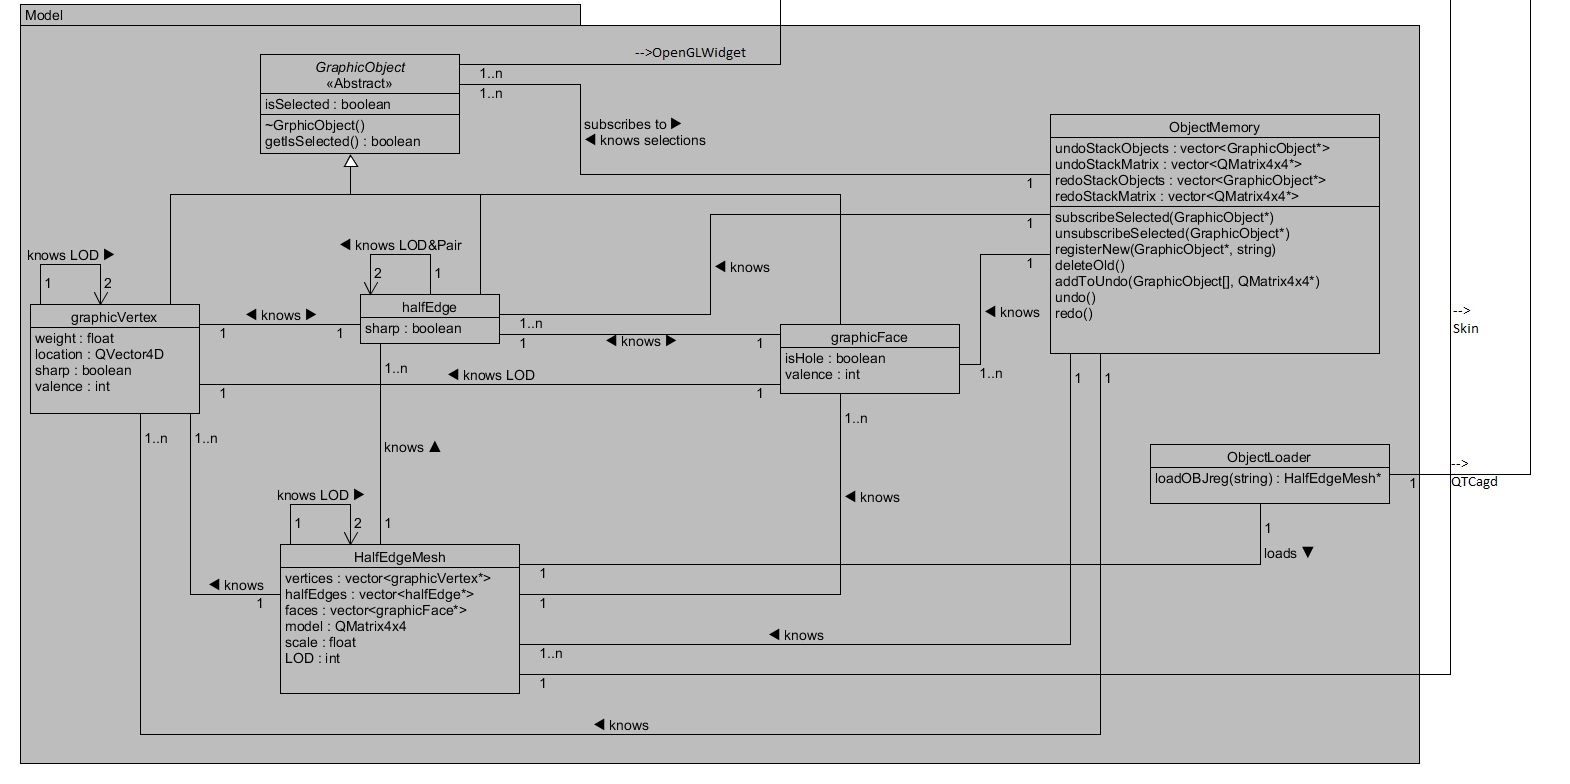
\includegraphics[angle=90,scale=0.5]{content/pictures/architekturModel.png}
\caption{Model-Paket der Architektur}
\label{fig:model}
\end{figure}

Wie bereits erwähnt stellt das Model in Abb. \ref{fig:model} unter anderem die HalfEdge-Struktur bereit. Hierzu dienen die Strukturen graphicVertex, halfEdge und graphicFace, welche alle von der abstrakten GraphicObject-Klasse erben. 
Dies erleichtert später die Verknüpfung der verschiedenen Level of Detail (LOD) nach Ausführungen von Unterteilungsalgorithmen. 
Zur einfacheren Datenhaltung werden die genannten Strukturen als HalfEdgeMesh-Klasse gespeichert, die alle Punkte, Kanten und Flächen eines Objektes enthält. 
Des Weiteren kennt das Mesh das momentane LOD. 

Die entsprechenden Objekte werden über die ObjectLoader-Klasse geladen.\\

Die ObjectMemory-Klasse ist zurzeit noch ungenutzt. 
Mit Verweis auf Kapitel \ref{chap:Ausblick} sollte an dieser Stelle z.B. eine Undo-Redo-Funktion realisiert werden. 
Dies wurde aufgrund von Zeitmangel jedoch nicht umgesetzt.

\subsubsection{View}
\begin{figure}[htbp]
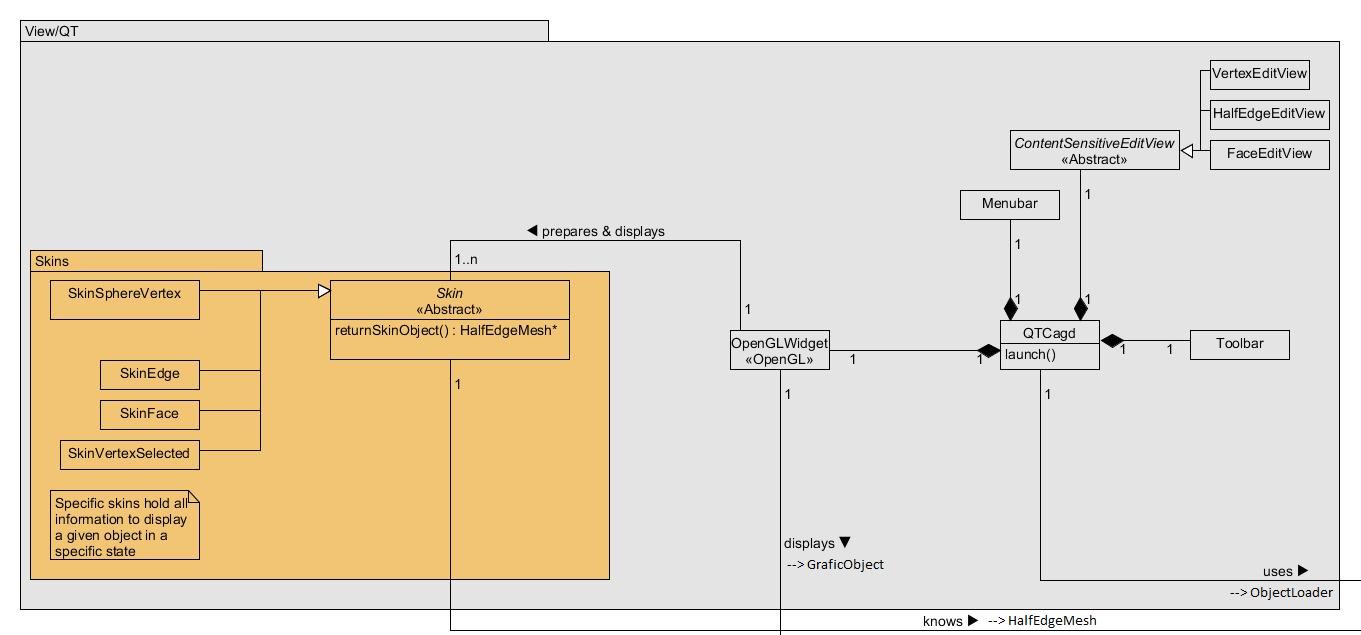
\includegraphics[angle=90,scale=0.6]{content/pictures/architekturView.png}
\caption{Model-Paket der Architektur}
\label{fig:view}
\end{figure}

Um den Aufwand für UI-Programmierung zu reduzieren, haben wir uns des QT-Frameworks bedient. 
Dem entsprechend besteht die View zum größten Teil aus externen QT-Abhängigkeiten. 
Das Hauptfenster der Anwendung wird in QTCagd realisiert, welche eine mit dem QT-Designer erstellte QTCagd.ui einbindet und anzeigt.
Des Weiteren werden dort entsprechende Signale für UI-Eingaben und Auswahlen gesendet.

Das OpenGLWidget hingegen ist ein Teil des Hauptfensters und kümmert sich um sämtliche OpenGL-spezifischen Anzeigen und Operationen.
Dies umfasst z.B. das Anzeigen von Vertices, Edges und Faces. 

Das Skin-Paket umfasst Objekte, die zum Anzeigen der internen GraficObjects genutzt werden. 
So existiert z.B ein Sphere-Model, das genutzt wird, um dem Nutzer im die Auswahl von Vertices zu erleichtern. 
Der ContextSensitiveEditView ist das Menü auf der rechten Seite in Abb. \ref{ui}. Dieses Menü ändert sich basierend auf der momentanen Auswahl.

\begin{figure}[htbp]
\centering
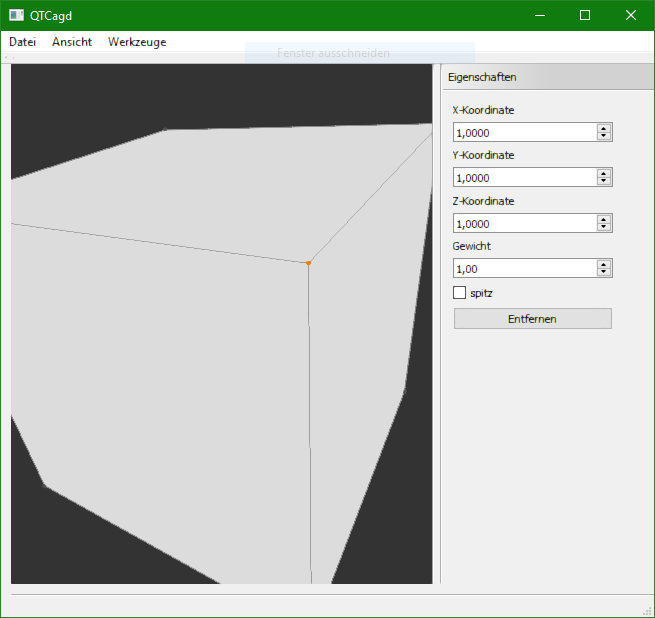
\includegraphics[scale=0.7]{content/pictures/cadgWindow.PNG}
\caption{UI der Anwendung}
\label{fig:ui}
\end{figure}


\section{Erklärung der Algorithmen}
\subsection{Catmull-Clark-Unterteilung}
Im Zuge des Projektes wurde der Catmull-Clark-Algorithmus für Unterteilungsflächen umgesetzt. 
Darauf soll in den folgenden Unterkapiteln genauer eingangen werden. 
Zuerst wird der allgemeine Fall betrachtet. 
Anschließend die Regelungen für scharfe Kanten und spitze Punkte. 
Abschließend wird noch kurz auf die Limitpunkte eingegangen.

\subsubsection{Allgemeiner Algorithmus}
Bei dem Algorithmus werden die Flächen des Meshes unterteilt. 
Dabei entsteht für jeden existierenden Punkt, jede Kante und jede Fläche ein neuer Punkt.
Dies funktioniert für beliebige Topologien. 
Nach der ersten Iteration des Algorithmus gibt es im Mesh nur noch Flächen mit Valenz vier.
Des Weiteren enstehen nach der ersten Iteration nurnoch Punkte mit Valenz vier. 
Die Anzahl der irregulären Punkte \emph{nach} der ersten Iteration bleibt gleich.

Die neuen Punkte werden nach folgenden Regeln gebildet:\\
\begin{itemize}
\item Ein neuer Flächenpunkt errechnet sich aus dem Mittel der die Fläche umschließenden Punkte.
\item Ein neuer Kantenpunkt wird aus dem Mittel der neuen Flächenpunkten und der angrenzenden Punkte der Kante gebildet.
\item Neue Eckpunkte werden aus den neuen, angrenzenden Flächenpunkten, den inzidenten Punkten und dem alten Eckpunkt errechnet.
\end{itemize}

Im folgenden wird auf die genauen Berechnungen eingangen.

\paragraph{Flächenpunkte}
\begin{figure}[htpb]
\centering
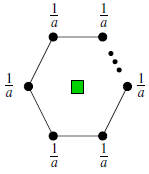
\includegraphics[scale=0.8]{content/pictures/facepoints.png}
\caption{Berechnung der Flächenpunkte}
\label{fig:facepoints}
\end{figure}

In Abb.~\ref{fig:facepoints} wird die Berechnung der neuen Flächenpunkte(grün) dargestellt. Die Variable \emph{a} bezeichnet die Flächenvalenz der jeweiligen Fläche.

\paragraph{Kantenpunkte}
\begin{figure}[htpb]
\centering
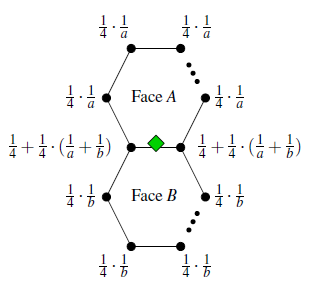
\includegraphics[scale=0.8]{content/pictures/edgepoints.png}
\caption{Berechnung der Kantenpunkte}
\label{fig:edgepoints}
\end{figure}

Die Kantenpunkte(grün) werden wie in Abb. ~\ref{fig:edgepoints} ermittelt. Die Variable \emph{a} bezeichnet die Flächenvalenz der Fläche A und die Variable \emph{b} entsprechend für Fläche B. Zu beachten ist hier der Spezialfall in Kap.~\ref{sec:sharpEdge}.

\paragraph{Eckpunkte}
\begin{figure}[htpb]
\centering
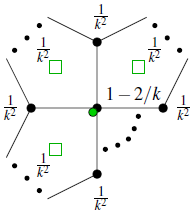
\includegraphics[scale=0.8]{content/pictures/vertexpoints.png}
\caption{Berechnung der Eckpunkte}
\label{fig:vertexpoints}
\end{figure}

Die neuen Eckpunkte ergeben sich durch Anteile der neuen Flächenpunkte und der alten, inzidenten Eckpunkte, wie in Abb.~\ref{fig:vertexpoints} dargestellt. Hierbei bezeichnet \emph{k} die Punktvalenz.

\subsubsection{Scharfe Kanten und spitze Punkte}
\label{sec:sharpEdge}
Eine scharfe Kante verwendet gesonderte Regeln um beim Unterteilen andere Ergebnisse zu erzielen. Dies begründet sich darin, dass bei der Berechnung nur die inzidenten Eckpunkte betrachtet werden. Es entstehen sichtbare Knicke im Mesh. \\

Ein spezieller Einsatzbereich der scharfen Kanten ist die Umrandung von Löchern im Mesh. Der Einsatz scharfer Kanten verhindert hierbei ein Anwachsen der Lochgröße.
\begin{figure}[tpb]
\centering
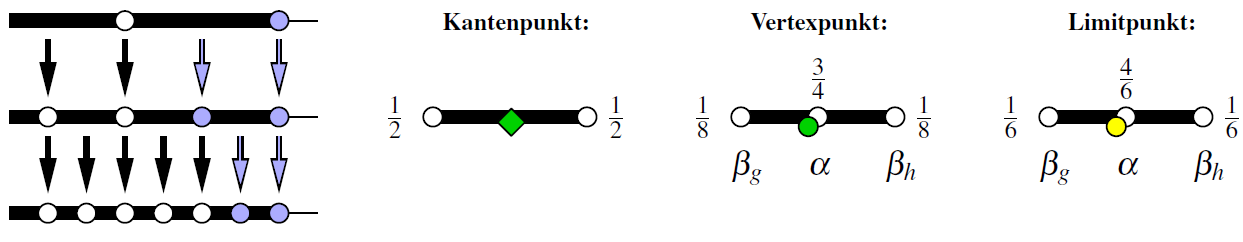
\includegraphics[width=\columnwidth]{content/pictures/sharpLimit.png}
\caption{Berechnung der scharfen Kanten mit Limitpunkten}
\label{fig:sharpLimit}
\end{figure}
Die Kantenpunkte und Eckpunkte, die auf einer scharfen Kante liegen, errechnen sich mit den in Abb.~\ref{fig:sharpLimit} gezeigten Verhältnissen. 

Ein spitzer Punkt erhält bei der Unterteilung durch Catmull-Clark seine Ursprungsposition.

\subsubsection{Limitpunkte}
Durch den Einsatz des Catmull-Clark Algorithmus schrumpft das unterteilte Mesh. Nach unendlich vielen Iterationen konvergiert das Mesh gegen eine Limitfläche. 
Für einen Punkt des Meshes lässt sich sein zugehöriger Punkt auf der Limitfläche bestimmen, die dazu benötigten Regeln heißen Limitpunktregeln.
\begin{figure}[htpb]
\centering
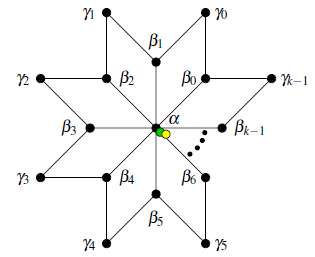
\includegraphics[scale=0.7]{content/pictures/limit.png}
\caption{Berechnung der Limitpunkte}
\label{fig:limit}
\end{figure}

Abb.~\ref{fig:limit} zeigt einen Ausschnitt aus einem Vierecksmesh.
Die Variablen $\alpha$ , $\beta$ und $\gamma$ beschreiben den Eckpunkt, seine inzidenten Eckpunkte und die Eckpunkte in Zweier-Nachbarschaft.  

In den Limitpunkt gehen die genannten Komponenten zu folgenden Verhältnissen ein. Hierbei bezeichnet \emph{k} die Punktvalenz und \emph{i} den i-ten inzidenten Punkt bzw. Punkt in Zweier-Nachbarschaft.
\begin{equation}
\alpha = 1-\dfrac{5}{k+5}\\
\beta_i = \dfrac{4}{(k+5)k}\\
\gamma_i = \dfrac{1}{(k+5)k}
\end{equation}

An scharfen Kanten gelten für die Berechnung von Limitpunkten die in Abb.~\ref{fig:sharpLimit} gezeigten Verhältnisse.

\subsection{Punktglättung}
Bei der Punktglättung werden alle Punkten, der zu einem Punkt inzidenten Flächen, mit dem Ursprungspunkt addiert. 
Aus dem Mittel ergibt sich der geglättete Punkt. 
Zwischen dem Ursprungspunkt und dem geglätteten Punkt kann man nun per Interpolation eine beliebige Glättungsstufe erhalten.

\subsection{Löschen von Punkten, Kanten und Flächen}
Im folgenden wird die Funktion, Punkte, Kanten und Flächen zu löschen näher betrachtet.
Insbesondere wird kurz auf Besonderheiten bei den einzelnen Verfahren hingewiesen.
\subsubsection{Löschen von Punkten}
Das Löschen von Punkten ist der schwierigste Fall beim Löschen. Hierbei müssen einige Schritte unternommen werden und auf einige Spezialfälle geachtet werden. 
Allgemein betrachtet muss folgendes geschehen:
\begin{itemize}
\item Der ausgewählte Punkt muss entfernt werden.
\item Alle inzidenten Kanten müssen entfernt werden.
\item Alle inzidenten Flächen müssen entfernt werden.
\item Die inzidenten Eckpunkte zeigen nicht mehr auf die entfernten Kanten.
\item Die Valenz der inzidenten Eckpunkte muss angepasst werden.
\item An der entsprechenden Stelle entstehen ein oder mehrere Löcher.
\item Die HalfEdge-Datenstruktur an der entsprechenden Stelle muss aktualisiert werden. Dabei muss die Konsistenz trotz entfernter Kanten und eines oder mehrerer neuer Löcher erhalten bleiben.
\end{itemize}

\subsubsection{Löschen von Kanten}
Das Löschen von Kanten ist dem Löschen eines Punktes recht ähnlich.
\begin{itemize}
\item Die entsprechende Kante (und damit die unterliegenden Halfedges) müssen entfernt werden. 
\item Die inzidenten Flächen werden entfernt und durch ein oder mehrere Löcher ersetzt.
\item Die Valenz der inzidenten Punkte muss entsprechend angepasst werden.
\item Die HalfEdge-Datenstruktur muss wie oben aktualisiert werden, um die Konsistenz zu erhalten.
\end{itemize}

\subsubsection{Löschen von Flächen}
Das Löschen einer Fläche ist der einfachste Fall.
Hierbei wird lediglich die Fläche durch ein Loch ersetzt und die HalfEdge-Datenstruktur mit scharfen Kanten versehen.



\section{Probleme bei der Entwicklung}
%Qt Neuland
%Qt Designer nicht gut in VS eingebunden
%Debugging in MS VS
%Performance
%Geeignete Architektur

Bei der Arbeit am Projekt sind wir nur auf wenige größere Probleme gestoßen. 
Die meisten Probleme, die wir hatten, hatten mit der Fehlerfindung in Visual Studio und C++ zu tun. 
An vielen Stellen war es nicht offensichtlich, an welcher Stelle nun ein Fehler auftrat und warum. 

Das Problem wurde insbesondere dadurch verstärkt, dass wir keinerlei Vorkenntnis mit QT hatten, welches wir für die UI nutzen wollten. 
Dies sollte uns einiges an Arbeit im Bereich der Oberflächengestaltung ersparen.
Im Endeffekt haben wir vermutlich das gleiche an Einarbeitungszeit aufwenden müssen. 
Des Weiteren hatten wir einige Probleme mit dem QT Designer Tool, welches schnelles und einfaches erstellen von UIs ermöglichen soll. 
Insbesondere dessen Visual Studio Einbindung funktioniert nicht immer, wie wir es erwartet hätten. 

Ein weiteres Problem war das Finden einer geeigneten und erweiterbaren Architektur für das Projekt. 
Insbesondere die Erweiterbarkeit war zu Anfang schwierig, da noch nicht alle Aufgaben und nötigen Funktionen bekannt waren.
Dem entsprechend hat die Architektur einige Iterationen gesehen.

Das letzte große Problem war die Performance. 
Mit wachsendem Funktionsumfang wurde das Projekt leider deutlich langsamer. 
Bei ``größeren`` Meshes -viele Vertices und Edges- dauerten dann Catmull-Clark Iterationen eine Minute oder länger, bei einem Model mit 50.000 Vertices und 300.000 Halfedges dauert selbst das Laden des Objektes etwa 30 Sekunden.



\section{Ausblick}
\label{chap:Ausblick}
Die Anwendung könnte auf mehrere Arten erweitert werden.
Zum einen wäre es möglich weitere Unterteilungsverfahren zu implementieren, wie z.B. Loop-Subdivide oder Doo-Sabin.
Andererseits wäre es natürlich auch möglich bestehende Funktionen auszubauen. 
So wäre das Löschen von Kanten und Flächen eine interessante Möglichkeit.
Des Weiteren könnte auch eine einfache Rotation des Meshes statt der Kamera stattfinden.
Außerdem könnte man noch eine einzige Fläche zur weiteren Verarbeitung (verschieben, löschen, scharf setzen,...) unterteilen lassen, statt das ganze Mesh zu unterteilen.
Eine abschließende Erweiterungsmöglichkeit wäre eine Extrude-Funktion, die es dem Nutzer erlaubt eine Fläche aus einer existierenden zu extrahieren, welche das Mesh fortsetzt.

Im Bereich der Optimierung liegt ganz klar die Performance im Fokus. 
Diese könnte vermutlich mit Techniken wie asynchroner Verarbeitung und Multithreading deutlich verbessert werden.
Leider war im Rahmen des Projektes keine Zeit für diese Schritte.


\section{Anleitung}
\subsection{Objekt-Dateien einlesen}
Unter $"$Datei->Öffnen$"$ kann eine Objekt-Datei geöffnet werden. (siehe ~\ref{fig:DateiOeffnen})
\begin{figure}[ht!]
\centering
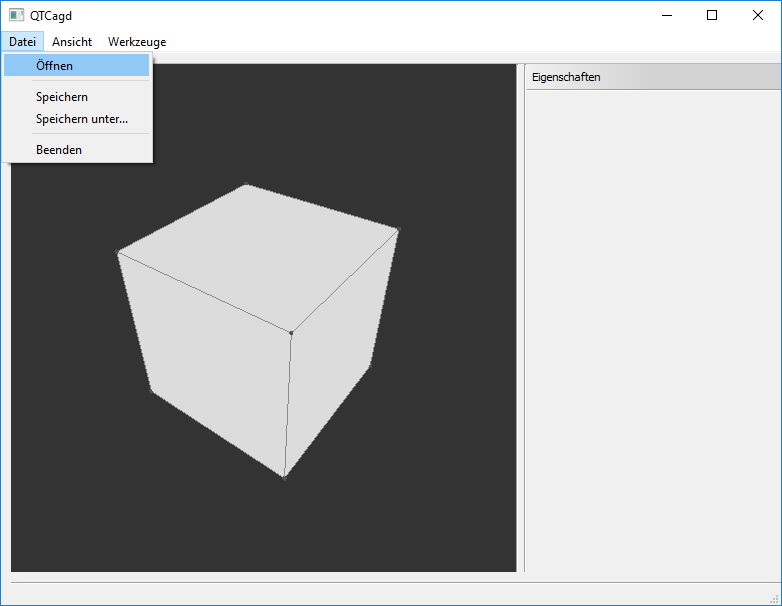
\includegraphics[width=0.6\linewidth]{content/pictures/0-DateiOeffnen}
\label{fig:DateiOeffnen}
\caption{}
\end{figure}
\subsection{Objekt-Dateien speichern}
Unter $"$Datei->Speichern$"$ oder mit $"$Datei->Speichern unter...$"$ kann eine Objekt-Datei gespeichert werden. (siehe ~\ref{fig:DateiSpeichern})

\begin{figure}[ht!]
	\centering
	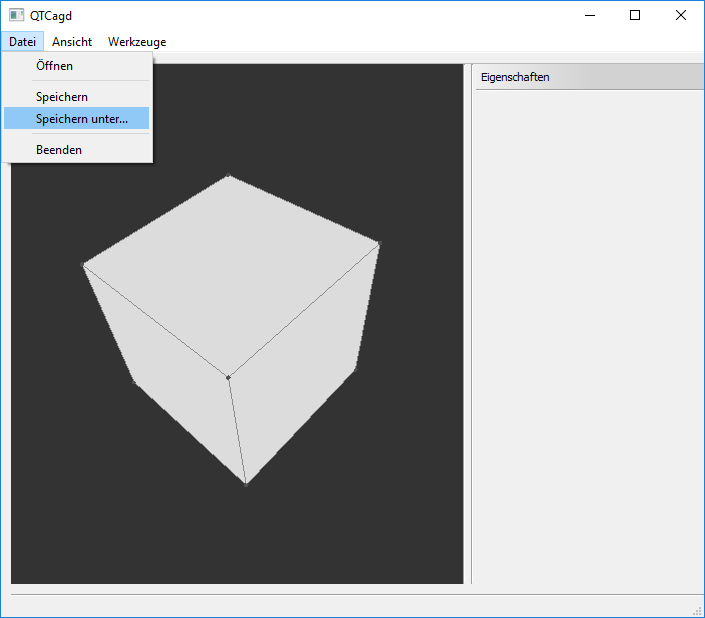
\includegraphics[width=0.6\linewidth]{content/pictures/1-DateiSpeichern}
	\label{fig:DateiSpeichern}
	\caption{}
\end{figure}

\subsection{Ansichtsmodi}
Es können 3 Ansichtsmodi aktiviert werden und zwar den $"$Vertex Mode$"$ oder den $"$Edge Mode$"$ oder den $"$Face Mode$"$. (siehe ~\ref{fig:Ansichtsmodi})\\
Punkte können im $"$Vertex Mode$"$ bearbeitet werden.\\
Kanten können im $"$Edge Mode$"$ bearbeitet werden.\\
Flächen können im $"$Face Mode$"$ bearbeitet werden.

\begin{figure}[ht!]
	\centering
	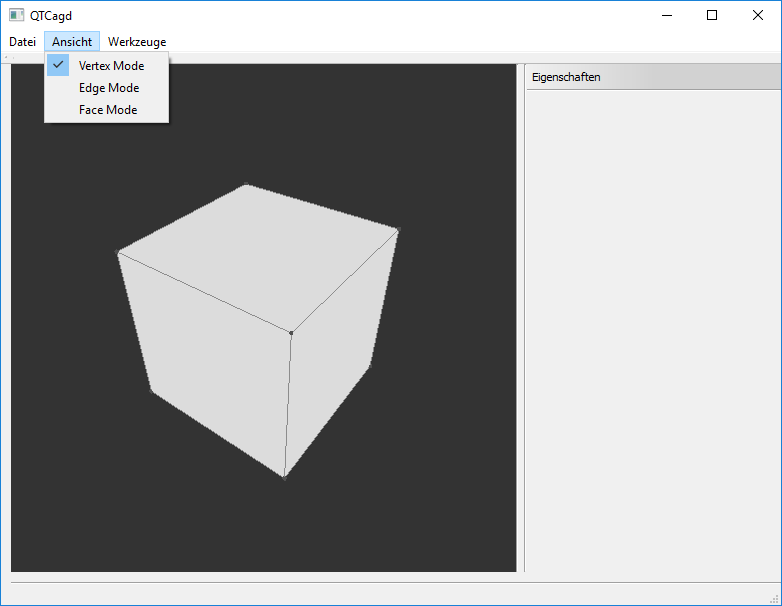
\includegraphics[width=0.6\linewidth]{content/pictures/2-Ansichtsmodi}
	\label{fig:Ansichtsmodi}
	\caption{}
\end{figure}

\subsection{Objekte selektieren}
Mit der Linken Maustaste können Grafikobjekte wie Punkte oder Kanten selektiert werden.\\
Mit Strg + Linke Maustaste kann eine Gruppe von Objekten selektiert werden.\\
Die Selektierten Objekte sind orange gefärbt.\\
Mit der Rechten Maustaste kann das ganze Mesh gedreht werden. (siehe ~\ref{fig:ObjekteSelektieren})\\

\begin{figure}[ht!]
	\centering
	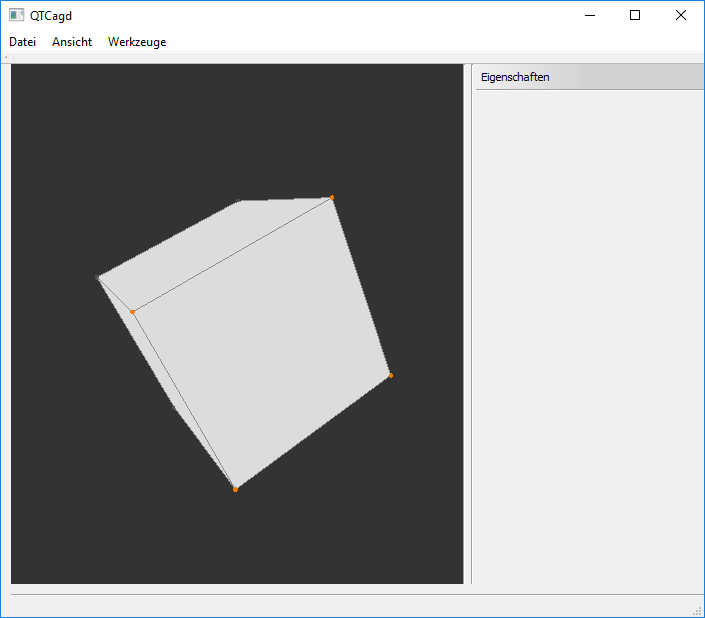
\includegraphics[width=0.6\linewidth]{content/pictures/3-ObjekteSelektieren}
	\label{fig:ObjekteSelektieren}
	\caption{}
\end{figure}

\subsection{Punkte verschieben}
Selektierte Punkte können mit gedrückter (linker) Maustaste verschoben werden.\\
Ein selektierter Punkt kann auch mit den Slidern im $"$Eigenschaften$"$ Menü verschoben werden.  (siehe ~\ref{fig:PunkteVerschieben})

\begin{figure}[ht!]
	\centering
	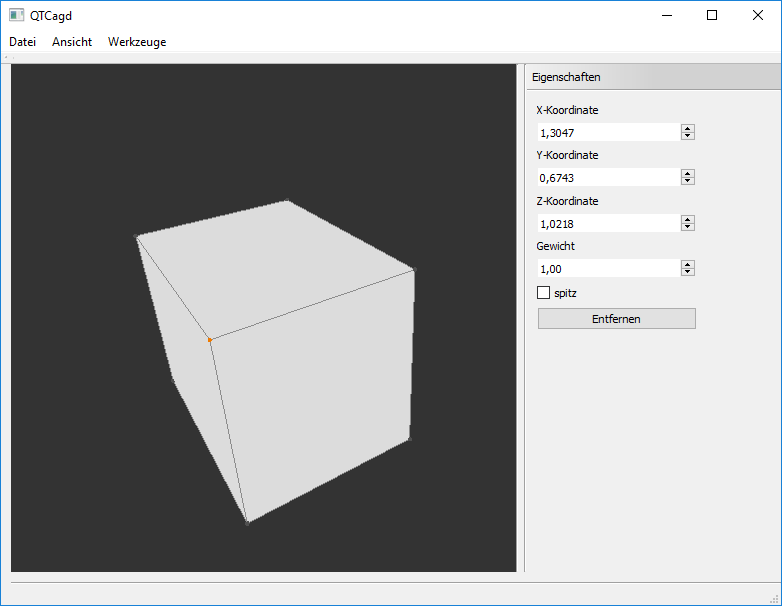
\includegraphics[width=0.6\linewidth]{content/pictures/4-PunkteVerschieben}
	\label{fig:PunkteVerschieben}
	\caption{}
\end{figure}

\subsection{Punkte löschen}
Selektierte Punkte können mit Entf gelöscht werden.
Ein selektierter Punkt kann auch mit den Button $"$Entfernen$"$ im $"$Eigenschaften$"$ Menü gelöscht werden.  (siehe ~\ref{fig:PunkteLoeschen})

\begin{figure}[ht!]
	\centering
	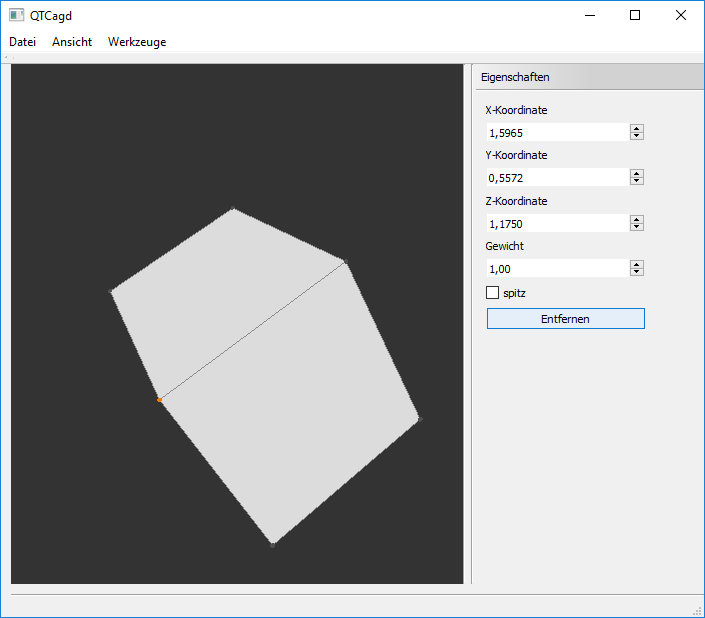
\includegraphics[width=0.6\linewidth]{content/pictures/5-PunkteLoeschen}
	\label{fig:PunkteLoeschen}
	\caption{}
\end{figure}

\subsection{Punkte gewichten}
Ein selektierter Punkt kann mit den Slider $"$Gewicht$"$ im $"$Eigenschaften$"$ Menü gewichtet werden.  (siehe ~\ref{fig:PunkteGewichten})

\begin{figure}[ht!]
	\centering
	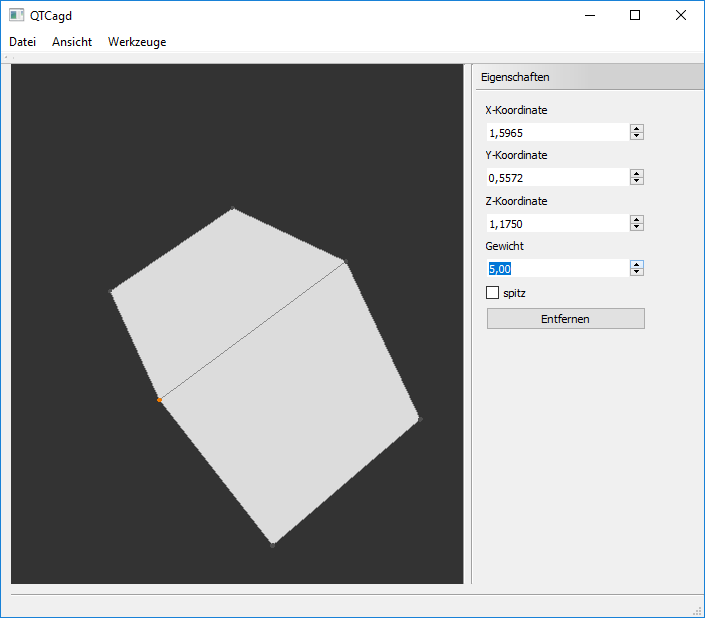
\includegraphics[width=0.6\linewidth]{content/pictures/6-PunkteGewichten}
	\label{fig:PunkteGewichten}
	\caption{}
\end{figure}

\subsection{Punkte und Kanten scharf setzen}
Ein selektierter Punkt oder selektierte Kante kann mit der Checkbox $"$spitz$"$ bzw. $"$scharf$"$ im $"$Eigenschaften$"$ Menü scharf gesetzt werden. (siehe ~\ref{fig:Punkte-KantenScharfSetzen})

\begin{figure}[ht!]
	\centering
	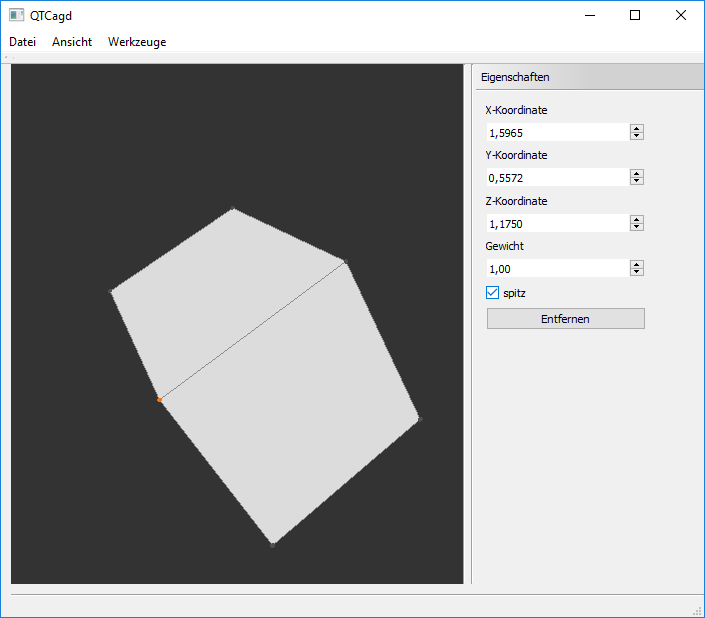
\includegraphics[width=0.6\linewidth]{content/pictures/7-Punkte-KantenScharfSetzen}
	\label{fig:Punkte-KantenScharfSetzen}
	\caption{}
\end{figure}

\subsection{Mesh mit Catmull-Clark unterteilen}
Unter $"$Werkzeuge->Catmull-Clark$"$ wird das $"$Catmull-Clark Subdivision$"$ Menü geöffnet.\\
Der Button $"$Anwenden$"$ unterteilt das Mesh. (siehe ~\ref{fig:MeshCatmullClark})

\begin{figure}[ht!]
	\centering
	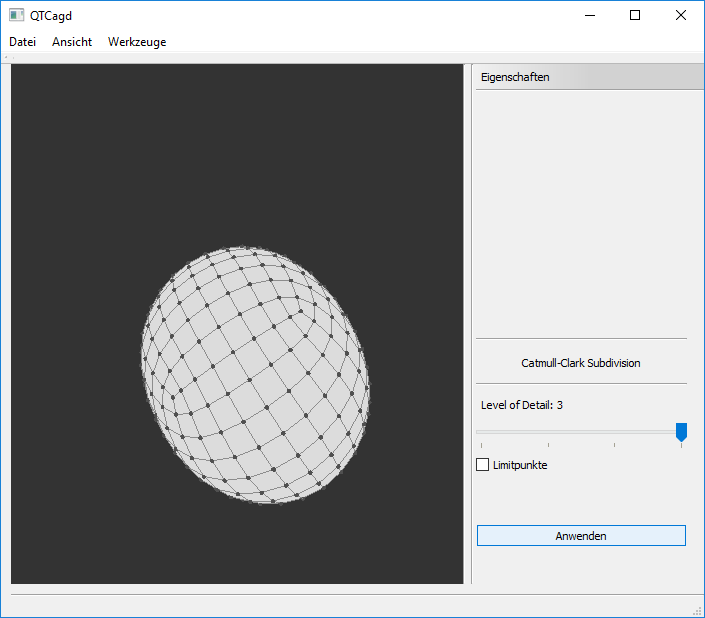
\includegraphics[width=0.6\linewidth]{content/pictures/8-MeshCatmullClark}
	\label{fig:MeshCatmullClark}
	\caption{}
\end{figure}

\subsection{Konsistenzprüfung und Statistik}
Mit der Taste $"$T$"$ kann ein Mesh auf Fehler untersucht werden und die Statistik angezeigt werden.\\
Außerdem wird nach jeder Iteration Catmull-Clark automatisch auf Fehler untersucht. (siehe ~\ref{fig:TestStatistik})

\begin{figure}[ht!]
	\centering
	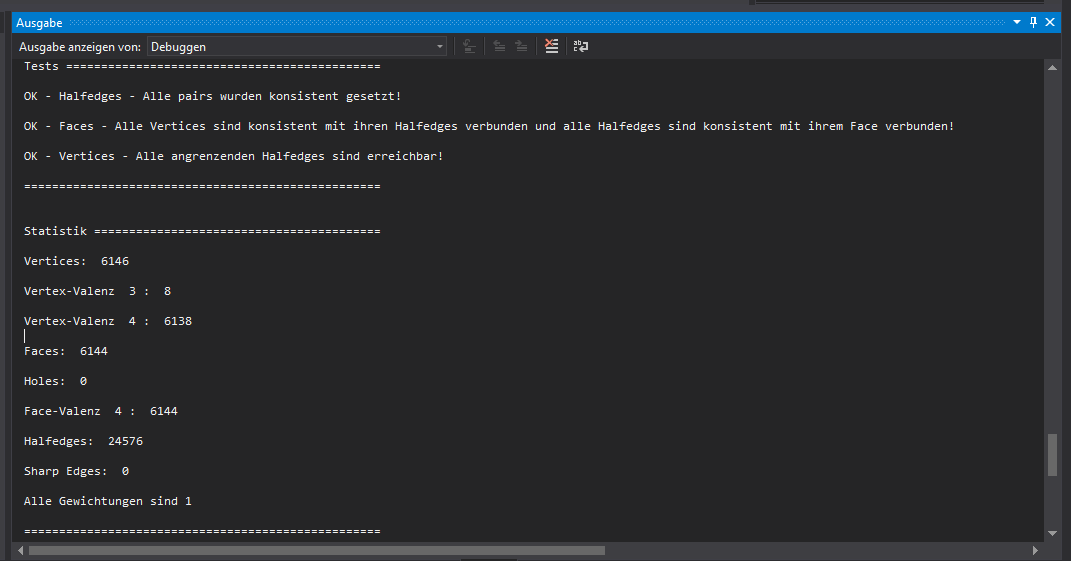
\includegraphics[width=0.6\linewidth]{content/pictures/9-TestStatistik}
	\label{fig:TestStatistik}
	\caption{}
\end{figure}


\end{document}
%% Dokument ENDE %%%%%%%%%%%%%%%%%%%%%%%%%%%%%%%%%%%%%%%%%%%%%%%%%%%%%%%%%%

